\pdfminorversion=3
\documentclass[tikz,border=1mm]{standalone}
\usepackage{alain}
\pagestyle{rien}


\begin{document}
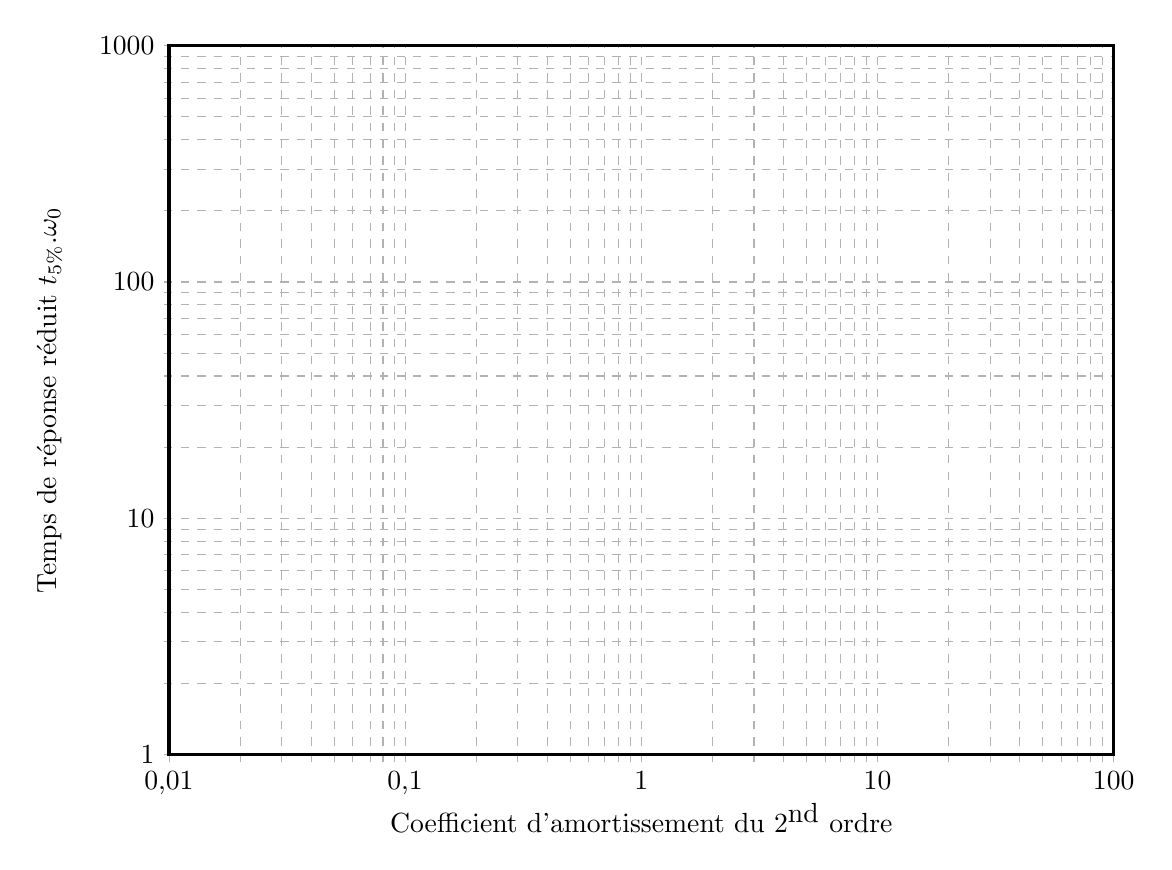
\begin{tikzpicture}[yscale=1,xscale=.6]
\foreach \x in {0.01,0.02,.03,.04,.05,.06,.07,.08,.09,0.1,0.2,0.3,0.4,0.5,0.6,0.7,0.8,0.9,1
,2,3,4,5,6,7,8,9,10,20,30,40,50,60,70,80,90,100} {
\draw[dashed,gray!60] ({log10(\x)*5},-0.1) -- ({log10(\x)*5},9);
}
\foreach \x in {1,2,3,4,5,6,7,8,9,10,20,30,40,50,60,70,80,90,100,200,300,400,500,600,700,800,900,1000} {
\draw[dashed,gray!60] (-10.1,{log10(\x)*3}) -- (10,{log10(\x)*3});
}
\node[below] at (-10,-.1) {\numprint{0,01}};
\node[below] at (-5,-.1) {\numprint{0,1}};
\node[below] at (0,-.1) {\numprint{1}};
\node[below] at (5,-.1) {\numprint{10}};
\node[below] at (10,-.1) {\numprint{100}};
\node[left] at (-10.1,0) {\numprint{1}};
\node[left] at (-10.1,3) {\numprint{10}};
\node[left] at (-10.1,6) {\numprint{100}};
\node[left] at (-10.1,9) {\numprint{1000}};
\node[below] at (0,-.5) {Coefficient d'amortissement du $2^\textrm{nd}$ ordre};
\node[below,rotate=90] at (-13.,4.5) {Temps de réponse réduit $t_{5\%}.\omega_0$};
\draw[xscale=5,yscale=3,very thick, color=black] plot file {images/abaque_tr5_0.01_100_log.table};
\draw[very thick] (-10,0) rectangle (10,9);
\end{tikzpicture}
\end{document}
